% Build: module load texlive/20240312-GCC-13.3.0 && pdflatex translation.tex (twice)
% Facts: research/rebuild/FEATURES.md ("Translation: putting the surveys on the PUF's terms"),
% research/rebuild/NEXT_STEPS.md (the 27 October mapping decisions), pipeline/fillin.py (the
% fill-in algorithm and its assumption), the 28 October rebuild talk (interest example: 2015 PUF
% against 2016 SCF, married, wages $75-200k), the 28 October overtime run's training log
% (SIPP shares with none, pass 53).

% Shared look, copied from ../2026-10_rebuild/rebuild_talk.tex (lines 1-75)

\documentclass[11pt,aspectratio=169]{beamer}

% ---------------------------------------------------------------------------
% Look: plain beamer, Yale colours
% ---------------------------------------------------------------------------
\usetheme{default}
\usefonttheme{professionalfonts}
\setbeamertemplate{navigation symbols}{}

\definecolor{yaleblue}{HTML}{00356B}
\definecolor{yalemid}{HTML}{286DC0}
\definecolor{yalelight}{HTML}{63AAFF}
\definecolor{yalegrey}{HTML}{4A4A4A}
\definecolor{yalelightgrey}{HTML}{DDDDDD}

\setbeamercolor{structure}{fg=yaleblue}
\setbeamercolor{normal text}{fg=black}
\setbeamercolor{frametitle}{fg=yaleblue}
\setbeamercolor{title}{fg=yaleblue}
\setbeamercolor{alerted text}{fg=yalemid}
\setbeamercolor{block title}{fg=white,bg=yaleblue}
\setbeamercolor{block body}{bg=yalelightgrey!40}

\setbeamerfont{frametitle}{series=\bfseries,size=\large}
\setbeamerfont{title}{series=\bfseries,size=\Large}

\setbeamertemplate{itemize items}[circle]
\setbeamertemplate{blocks}[rounded][shadow=false]

% A thin blue rule under each frame title
\setbeamertemplate{frametitle}{%
  \vspace*{0.6em}%
  \usebeamerfont{frametitle}\usebeamercolor[fg]{frametitle}\insertframetitle\par
  \vspace*{-0.2em}{\color{yaleblue}\rule{\textwidth}{0.6pt}}%
}

% Footer: short title on the left, slide number on the right
\setbeamertemplate{footline}{%
  \hspace*{1.2em}{\color{yalegrey}\scriptsize\insertshorttitle}%
  \hfill{\color{yalegrey}\scriptsize\insertframenumber}\hspace*{1.2em}%
  \vspace*{0.6em}%
}

% ---------------------------------------------------------------------------
% Packages
% ---------------------------------------------------------------------------
\usepackage[T1]{fontenc}
\usepackage{lmodern}
\usepackage{booktabs}
\usepackage{array}
\usepackage{graphicx}
\usepackage{amsmath}
\usepackage{tikz}
\usetikzlibrary{positioning,arrows.meta,calc}
\usepackage{pgfplots}
\pgfplotsset{compat=1.18}
\graphicspath{{figures/}}

% Diagram styles
\tikzset{
  tok/.style={draw=yaleblue, rounded corners=2pt, font=\small, inner sep=4pt,
              minimum height=0.65cm},
  blank/.style={tok, fill=yalelight!35, font=\small\bfseries},
  box/.style={draw=yaleblue, rounded corners=2pt, font=\scriptsize, align=center,
               text width=2.1cm, minimum height=1.1cm, inner sep=3pt},
  arr/.style={-{Stealth[length=5pt]}, yaleblue, thick},
  cF/.style={fill=yaleblue},
  cP/.style={fill=yalelight!60},
  cN/.style={fill=white},
}

\pgfplotsset{colormap={yalemap}{color=(white) color=(yalelight) color=(yaleblue)}}



\newcommand{\slidenote}[1]{\par\vfill{\scriptsize\color{yalegrey}#1}}

\title{Translating survey records into tax-return terms}
\author{John Ricco}
\institute{The Budget Lab at Yale}
\date{October 2026}

\hyphenpenalty=10000
\exhyphenpenalty=10000

\begin{document}

\begin{frame}[plain,noframenumbering]
  \titlepage
\end{frame}

% ---------------------------------------------------------------------------
\begin{frame}{The problem}
  \begin{itemize}
    \item The model is estimated on the PUF and four surveys together: the SCF, CEX, CPS and SIPP.
          Variables that appear in several sources, such as wages, interest and Social Security,
          are estimated from all of them.
    \vspace{0.5em}
    \item The surveys do not measure these variables the way a tax return does.
    \begin{itemize}
      \item Definitions differ. CPS wages are before pre-tax deductions such as 401(k)
            contributions.
      \item Amounts are top-coded or misreported.
      \item Small amounts often go unreported.
    \end{itemize}
    \vspace{0.5em}
    \item Without a correction, the model would learn a mixture of the survey's concept and the tax
          return's. Variables found only in surveys, such as wealth, would be estimated conditional
          on the wrong amounts.
  \end{itemize}
\end{frame}

% ---------------------------------------------------------------------------
\begin{frame}{Example: interest income}
  \centering
  \begin{tikzpicture}
    \begin{axis}[ybar, width=12cm, height=5.4cm, bar width=14pt, ymin=0, ymax=32,
        symbolic x coords={\$1--100, \$100--500, \$500--2k, \$2k--10k, \$10k+},
        xtick=data, xticklabel style={font=\small}, yticklabel style={font=\small},
        ylabel={Per 100 tax units}, ylabel style={font=\small},
        xlabel={Interest received in the year}, xlabel style={font=\small},
        legend style={font=\small, draw=none, at={(0.97,0.95)}, anchor=north east},
        axis x line*=bottom, axis y line*=left, enlarge x limits=0.12,
        nodes near coords, every node near coord/.append style={font=\scriptsize}]
      \addplot[fill=yaleblue, draw=none] coordinates
        {(\$1--100,28) (\$100--500,13) (\$500--2k,4) (\$2k--10k,2) (\$10k+,1)};
      \addplot[fill=yalelight!70, draw=none] coordinates
        {(\$1--100,8) (\$100--500,6) (\$500--2k,3) (\$2k--10k,3) (\$10k+,1)};
      \legend{PUF: reported on the return (48 in total), SCF: reported in the survey (21 in total)}
    \end{axis}
  \end{tikzpicture}

  \vspace{0.3em}
  The gap is in small amounts, which many households do not report in the survey.
  Above \$2,000 the two sources agree.
  \slidenote{Married couples with wages of \$75,000--200,000. 2015 PUF and 2016 SCF (tax year 2015), weighted.}
\end{frame}

% ---------------------------------------------------------------------------
\begin{frame}{Two steps}
  \begin{enumerate}
    \item \textbf{A mapping function for each survey variable.} We look at how the survey's
          variable differs from the tax return's and choose a mapping by hand. It is applied
          once, before the model is estimated.
    \vspace{0.8em}
    \item \textbf{A fill-in for units that report zero.} Some units that report zero in the survey
          would show an amount on a tax return. The fill-in assigns amounts to some of them. It is
          applied while the model is estimated.
  \end{enumerate}
  \vspace{1em}
  Both steps compare each survey with the tax data for the same year: the PUF's filers, grown to
  that year, plus the non-filers from the CPS.
\end{frame}

% ---------------------------------------------------------------------------
\begin{frame}{Step 1: mapping functions}
  \small
  \renewcommand{\arraystretch}{1.3}
  \begin{tabular}{>{\raggedright}p{3.6cm} >{\raggedright}p{3.9cm} >{\raggedright\arraybackslash}p{5.2cm}}
    \toprule
    Kind of difference & Mapping & Example \\
    \midrule
    None & Keep the reported dollars & SCF interest and dividends \\
    A known difference in definition & Apply the tax rule & SCF capital losses held to the \$3,000 a return allows \\
    The order of units is right but the dollar scale is not & Percentile among holders & SCF and CPS wages; CPS dividends \\
    Reliable for small amounts, not at the top & Keep the dollars below a line, percentile above it & SIPP dividends, with a line at \$50,000 \\
    \bottomrule
  \end{tabular}
\end{frame}

% ---------------------------------------------------------------------------
\begin{frame}{Step 1 example: wages by percentile}
  \begin{itemize}
    \item CPS wages include pre-tax deductions, and the CPS has more high earners than tax returns
          show. In 2019 it has 29.0 million units with wages above \$100,000, against 21.9 million
          in the tax data.
    \vspace{0.5em}
    \item The mapping keeps the CPS's ranking of earners and takes the dollar amounts from the
          tax data.
    \vspace{0.5em}
    \item A CPS unit at the 90th percentile among CPS earners is given the wages of the unit at the
          90th percentile among earners in the tax data.
    \vspace{0.5em}
    \item The assumption is that the survey ranks earners correctly even where its dollar amounts
          are off.
  \end{itemize}
  \slidenote{Units with no wages are handled by step 2.}
\end{frame}

% ---------------------------------------------------------------------------
\begin{frame}{Step 2: two versions of each filled-in variable}
  \centering
  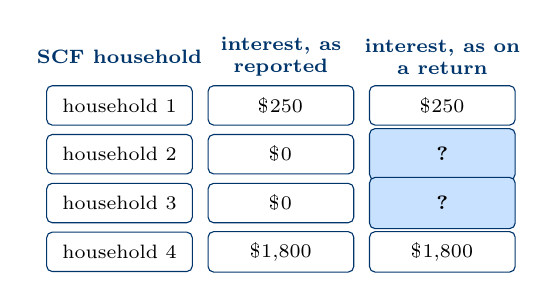
\begin{tikzpicture}[x=2.05cm, y=0.62cm,
      c/.style={tok, minimum width=1.85cm, minimum height=0.5cm, font=\scriptsize}]
    \node[font=\scriptsize\bfseries, text=yaleblue] at (1,0) {SCF household};
    \node[font=\scriptsize\bfseries, text=yaleblue, align=center] at (2,0) {interest, as\\reported};
    \node[font=\scriptsize\bfseries, text=yaleblue, align=center] at (3,0) {interest, as on\\a return};
    \foreach \r/\said/\ret/\hd in {1/\$250/\$250/0, 2/\$0/?/1, 3/\$0/?/1, 4/{\$1,800}/{\$1,800}/0} {
      \node[c] at (1,-\r) {household \r};
      \node[c] at (2,-\r) {\said};
      \ifnum\hd=1 \node[c, blank, font=\scriptsize\bfseries] at (3,-\r) {\ret}; \else \node[c] at (3,-\r) {\ret}; \fi
    }
  \end{tikzpicture}

  \vspace{0.4em}
  \raggedright
  \small
  \begin{itemize}
    \item The survey answer is kept and never changed.
    \item The tax-return version equals the answer for units that report an amount. For units that
          report zero it is drawn.
    \item PUF records have only the tax-return version. The model learns the tax-return version from
          all sources.
  \end{itemize}
\end{frame}

% ---------------------------------------------------------------------------
\begin{frame}{Step 2: assumptions}
  Within a type of unit (married or not, number of dependents, wage band):
  \vspace{0.4em}
  \begin{enumerate}
    \item The tax data gives the true share of units with an amount in each size range.
    \vspace{0.3em}
    \item A unit that reports an amount reports it correctly. Only zeros can be wrong.
    \vspace{0.3em}
    \item Whether a holder reports depends only on its type and the size of its amount. Two
          couples of the same type with \$50 of interest are equally likely to leave it out,
          whatever else is on their records.
  \end{enumerate}
  \vspace{0.6em}
  Under these assumptions, the reporting rate for size range $k$ is the survey's share over the tax
  data's share, $r_k = B_k / A_k$. In the interest example, for \$1--100 it is $8 / 28 = 0.29$.
\end{frame}

% ---------------------------------------------------------------------------
\begin{frame}{Step 2: the chance a zero-reporter holds an amount}
  \small
  For a zero-reporter with record $x$, Bayes' rule gives the chance that it holds an amount in
  range $k$:
  \[
    \Pr(\text{holds } k \mid \text{reports } 0, x)
    = \frac{\Pr(\text{holds } k \mid x)\,(1 - r_k)}{\Pr(\text{reports } 0 \mid x)}
    = \frac{C_k(x)\,\big(A_k / B_k - 1\big)}{C_0(x)}
  \]
  \begin{itemize}
    \item $C_k(x)$ is the model's probability that a unit with record $x$ reports an amount in range
          $k$. $C_0(x)$ is its probability of reporting zero.
    \item By assumption 3, $\Pr(\text{holds } k \mid x) = C_k(x) / r_k$, which gives the second
          equality.
    \item $A_k / B_k - 1$ is the number of hidden holders per reporter in the unit's type. It sets
          how many amounts are filled in.
    \item $C_k(x)$ sets which units receive them: those whose other answers look like reporters'.
  \end{itemize}
  \slidenote{$A_k$: the tax data's share in range $k$, by type. $B_k$: the average of $C_k(x)$ over the
             survey's units of that type. The total chance is capped at 100 percent.}
\end{frame}

% ---------------------------------------------------------------------------
\begin{frame}{Step 2 example: interest for married couples}
  \begin{columns}[T]
    \begin{column}{0.42\textwidth}
      \centering
      \small
      \begin{tabular}{lrrr}
        \toprule
        Per 100 couples & Tax data & SCF & Filled in \\
        \midrule
        \$1--100      & 28 & 8 & 20 \\
        \$100--500    & 13 & 6 & 7 \\
        \$500--2k     & 4  & 3 & 2 \\
        \$2k and over & 3  & 3 & 0 \\
        \midrule
        Any           & 48 & 21 & 28 \\
        \bottomrule
      \end{tabular}
    \end{column}
    \begin{column}{0.55\textwidth}
      \small
      A typical couple of this type, for \$1--100:
      \begin{itemize}
        \item $C_1 = 0.08$ and $C_0 = 0.79$
        \item hidden holders per reporter: $28/8 - 1 = 2.5$
        \item chance: $0.08 \times 2.5 / 0.79 = 0.25$
      \end{itemize}
      \vspace{0.3em}
      A couple with large savings and stock holdings might have $C_1 = 0.20$ and $C_0 = 0.55$.
      Its chance is $0.20 \times 2.5 / 0.55 = 0.91$.
    \end{column}
  \end{columns}
  \slidenote{Married couples with wages of \$75,000--200,000; 2015 PUF and 2016 SCF, weighted.
             The second couple's probabilities are made up for illustration.}
\end{frame}

% ---------------------------------------------------------------------------
\begin{frame}{Step 2 within pretraining}
  \small
  \begin{enumerate}
    \item \textbf{Passes 1 and 2.} No amounts are filled in.
    \vspace{0.3em}
    \item \textbf{At the start of each later pass}, for every filled-in variable and survey:
    \begin{itemize}
      \item $A_k$ by type, from the tax data for the survey's year;
      \item $C_k(x)$ for every survey unit, from the model's current parameters, with the
            tax-return versions hidden;
      \item $B_k$, the average of $C_k(x)$ within each type;
      \item each zero-reporter's chance of holding an amount in each range.
    \end{itemize}
    \vspace{0.3em}
    \item \textbf{In each batch}, new amounts are drawn for the zero-reporters from these chances.
          The parameters are then updated on the tax-return version.
  \end{enumerate}
  \vspace{0.4em}
  The chances use only survey answers and the tax data, never earlier fill-ins. As the model
  improves, it gets better at telling which zero-reporters look like holders.
\end{frame}

% ---------------------------------------------------------------------------
\begin{frame}{Checking the result}
  Share of SIPP units with none, 2019, during the 28 October run:
  \vspace{0.6em}
  \begin{center}
  \begin{tabular}{lrrr}
    \toprule
    & As reported & After the fill-in & Tax data \\
    \midrule
    Wages     & 30.5\% & 21.2\% & 22.5\% \\
    Dividends & 86.0\% & 79.6\% & 80.4\% \\
    \bottomrule
  \end{tabular}
  \end{center}
  \vspace{0.6em}
  \begin{itemize}
    \item A report compares each variable as reported, after step 1, after step 2 and in the tax
          data, for every survey and year.
    \item The fill-in is applied to wages, interest, dividends, capital gains, pensions, business
          income and Schedule E, among others, in each survey that measures them.
  \end{itemize}
  \slidenote{The tax-data figures are taken at the SIPP's mix of household types.}
\end{frame}

\end{document}
